\documentclass{standalone}

% graphics
\usepackage{tikz}
\usepackage{pgfplots}
\usepackage{siunitx}

\begin{document}

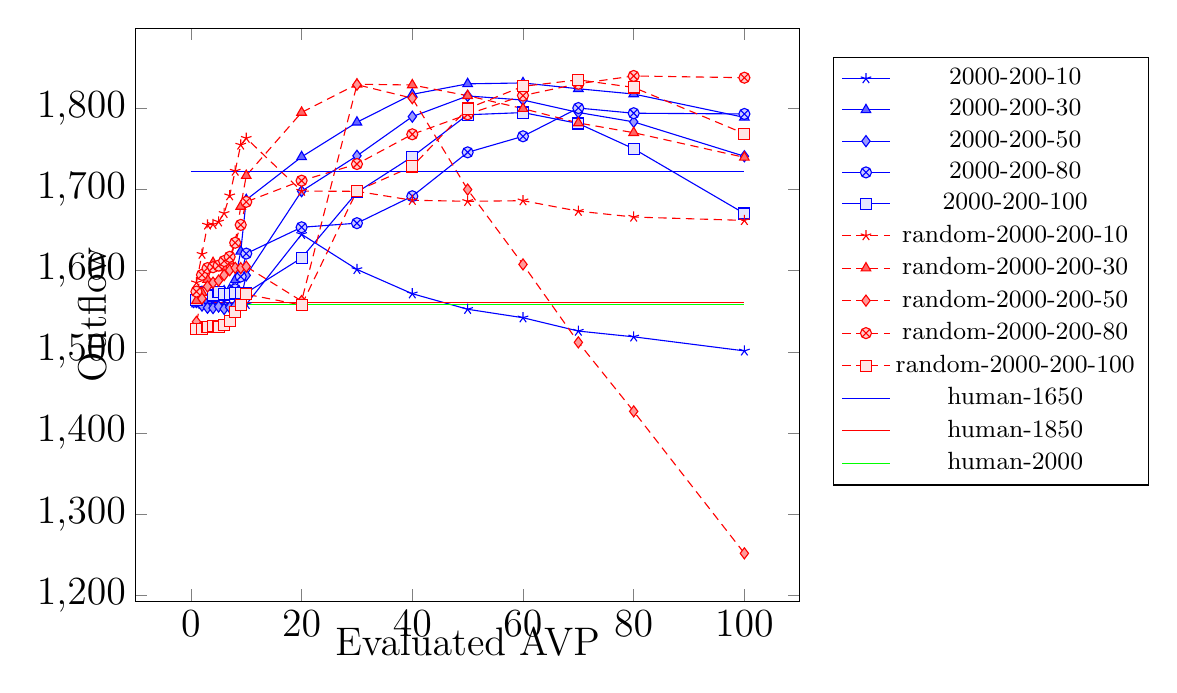
\begin{tikzpicture}[scale=1]
  \pgfplotsset{
      scale only axis,
      every x tick label/.append style={font=\Large},
      every y tick label/.append style={font=\Large},
	legend style={at={(1.05,0.95)},anchor=north west}
  }

\pgfplotscreateplotcyclelist{mycolorlist}{%
	blue,every mark/.append style={fill=blue!80}, mark=star, error bars/.cd, y dir=both, y explicit\\%
	blue,every mark/.append style={fill=blue!60}, mark=triangle*, error bars/.cd, y dir=both, y explicit\\%
	blue,every mark/.append style={fill=blue!40}, mark=diamond*, error bars/.cd, y dir=both, y explicit\\%
	blue,every mark/.append style={fill=blue!20}, mark=otimes*, error bars/.cd, y dir=both, y explicit\\%
	blue,every mark/.append style={fill=blue!10}, mark=square*, error bars/.cd, y dir=both, y explicit\\%
	red,densely dashed,every mark/.append style={solid,fill=red!80}, mark=star, error bars/.cd, y dir=both, y explicit\\%
	red,densely dashed,every mark/.append style={solid,fill=red!60},mark=triangle*, error bars/.cd, y dir=both, y explicit\\%
	red,densely dashed,every mark/.append style={solid,fill=red!40},mark=diamond*, error bars/.cd, y dir=both, y explicit\\%
	red,densely dashed,every mark/.append style={solid,fill=red!20}, mark=otimes*, error bars/.cd, y dir=both, y explicit\\%
	red,densely dashed,every mark/.append style={solid,fill=red!10}, mark=square*, error bars/.cd, y dir=both, y explicit\\%
	green!40!black, dashed,every mark/.append style={solid,fill=green!80}, mark=star, error bars/.cd, y dir=both, y explicit\\%
	green!40!black, dashed,every mark/.append style={solid,fill=green!60},mark=triangle*, error bars/.cd, y dir=both, y explicit\\%
	green!40!black, dashed,every mark/.append style={solid,fill=green!40},mark=diamond*, error bars/.cd, y dir=both, y explicit\\%
	green!40!black, dashed,every mark/.append style={solid,fill=green!20},mark=otimes*, error bars/.cd, y dir=both, y explicit\\%
	green!40!black, dashed,every mark/.append style={solid,fill=green!10},mark=square*, error bars/.cd, y dir=both, y explicit\\%
	black, dashed,every mark/.append style={solid,fill=green!80}, mark=star, error bars/.cd, y dir=both, y explicit\\%
	black, dashed,every mark/.append style={solid,fill=green!60},mark=triangle*, error bars/.cd, y dir=both, y explicit\\%
	black, dashed,every mark/.append style={solid,fill=green!40},mark=diamond*, error bars/.cd, y dir=both, y explicit\\%
	black, dashed,every mark/.append style={solid,fill=green!20},mark=otimes*, error bars/.cd, y dir=both, y explicit\\%
	black, dashed,every mark/.append style={solid,fill=green!10},mark=square*, error bars/.cd, y dir=both, y explicit\\%
	}


\begin{axis}[
    legend style={font=\small},
	ylabel={\Large Outflow},
	x label style={at={(axis description cs:0.5,-0.03)},anchor=north},
	y label style={at={(axis description cs:-0.030,0.5)}, anchor=south},
	xlabel={\Large Evaluated AVP},
	cycle list name=mycolorlist
]

\addplot table [x=a, y=b] {
a	 b	 c
1	1559.41	13.96
2	1558.51	14.17
3	1558.51	14.23
4	1558.22	13.62
5	1558.33	14.33
6	1558.01	14.39
7	1558.98	13.81
8	1557.83	14.44
9	1557.76	14.92
10	1558.44	14.7
20	1644.77	21.96
30	1601.53	20.31
40	1571.58	18.37
50	1552.43	17.99
60	1541.99	21.23
70	1525.57	23.97
80	1518.48	23.84
100	1501.16	22.65
};
\label{2000-200-10}

\addplot table [x=a, y=b] {
a	 b	 c
1	1558.69	13.78
2	1561.21	14.85
3	1563.12	15.12
4	1575.65	17.59
5	1573.49	16.79
6	1574.82	17.59
7	1576.58	16.1
8	1588.72	20.63
9	1623.74	29.56
10	1687.28	29.1
20	1740.13	43.95
30	1782.76	47.54
40	1817.21	49.04
50	1830.13	40.78
60	1831.21	31.01
70	1824.05	28.0
80	1817.57	29.46
100	1788.77	22.9
};
\label{2000-200-30}

\addplot table [x=a, y=b] {
a	 b	 c
1	1561.39	15.28
2	1556.96	14.5
3	1554.26	13.76
4	1553.9	12.38
5	1555.78	15.14
6	1552.82	14.2
7	1554.8	16.27
8	1556.78	13.38
9	1564.74	18.42
10	1594.19	25.2
20	1697.87	36.76
30	1741.46	52.91
40	1789.7	53.25
50	1815.23	38.07
60	1810.15	32.06
70	1794.85	30.47
80	1783.26	27.14
100	1740.89	28.81
};
\label{2000-200-50}

\addplot table [x=a, y=b] {
a	 b	 c
1	1565.06	14.74
2	1574.14	17.18
3	1574.71	18.69
4	1571.87	15.84
5	1571.04	16.52
6	1568.7	15.65
7	1571.69	18.34
8	1577.02	19.8
9	1592.75	22.69
10	1621.01	31.6
20	1653.41	29.71
30	1658.48	49.88
40	1691.64	54.89
50	1745.71	62.86
60	1765.48	53.96
70	1800.29	52.79
80	1793.92	45.84
100	1793.02	37.2
};
\label{2000-200-80}

\addplot table [x=a, y=b] {
a	 b	 c
1	1563.95	15.72
2	1571.04	18.16
3	1572.37	18.01
4	1569.38	17.07
5	1573.96	18.34
6	1570.68	18.14
7	1570.97	17.29
8	1572.48	16.85
9	1572.77	17.7
10	1572.73	18.42
20	1615.61	33.6
30	1696.5	31.65
40	1740.31	46.39
50	1792.04	47.67
60	1794.71	37.48
70	1781.28	32.96
80	1750.1	20.55
100	1670.4	28.19
};
\label{2000-200-100}

\addplot table [x=a, y=b] {
a	 b	 c
1	1585.22	16.34
2	1620.29	22.01
3	1656.32	21.79
4	1657.04	20.12
5	1660.18	24.4
6	1670.65	25.39
7	1692.36	29.95
8	1722.71	35.8
9	1754.82	27.65
10	1763.17	33.34
20	1698.01	49.2
30	1697.69	48.69
40	1686.71	60.86
50	1685.41	62.15
60	1686.17	58.38
70	1673.28	62.2
80	1666.04	60.38
100	1661.87	59.93
};
\label{random-2000-200-10}

\addplot table [x=a, y=b] {
a	 b	 c
1	1562.98	15.39
2	1572.95	16.06
3	1589.0	16.58
4	1609.74	18.1
5	1604.7	17.25
6	1603.19	18.2
7	1611.58	19.99
8	1634.47	25.83
9	1679.0	31.68
10	1717.02	27.18
20	1794.89	51.37
30	1829.63	37.29
40	1828.69	30.14
50	1815.48	25.79
60	1799.6	20.37
70	1781.93	25.96
80	1769.94	21.21
100	1739.52	18.01
};
\label{random-2000-200-30}

\addplot table [x=a, y=b] {
a	 b	 c
1	1536.98	19.51
2	1565.6	26.31
3	1580.51	21.67
4	1585.26	20.32
5	1587.74	15.65
6	1594.51	19.2
7	1600.56	18.43
8	1603.48	21.28
9	1603.15	23.3
10	1604.95	19.65
20	1562.54	23.41
30	1829.05	39.02
40	1812.46	18.23
50	1699.88	15.85
60	1607.65	14.78
70	1511.64	14.79
80	1426.64	14.48
100	1251.76	13.48
};
\label{random-2000-200-50}

\addplot table [x=a, y=b] {
a	 b	 c
1	1574.21	16.99
2	1594.8	14.29
3	1603.15	17.87
4	1604.2	16.74
5	1606.21	14.78
6	1611.86	17.85
7	1617.01	17.35
8	1634.36	24.43
9	1656.36	22.18
10	1684.73	24.63
20	1710.83	30.6
30	1731.31	37.82
40	1767.96	41.96
50	1792.51	49.13
60	1815.7	46.31
70	1830.24	39.38
80	1839.82	33.49
100	1837.66	27.01
};
\label{random-2000-200-80}

\addplot table [x=a, y=b] {
a	 b	 c
1	1528.02	19.88
2	1527.98	21.76
3	1530.36	20.5
4	1531.3	21.08
5	1530.79	24.19
6	1532.88	24.86
7	1537.52	24.18
8	1549.48	28.35
9	1557.18	25.56
10	1570.93	22.7
20	1557.58	14.6
30	1698.26	29.9
40	1728.36	27.49
50	1799.71	46.18
60	1827.07	42.03
70	1834.99	37.36
80	1825.7	32.94
100	1768.75	25.55
};
\label{random-2000-200-100}

\addplot[blue, samples=200] coordinates {(0,1722.200000) (100,1722.200000)};\label{human-1650}\addplot[red, samples=200] coordinates {(0,1560.380000) (100,1560.380000)};\label{human-1850}\addplot[green, samples=200] coordinates {(0,1558.120000) (100,1558.120000)};\label{human-2000}\addlegendimage{/pgfplots/refstyle=2000-200-10}
\addlegendentry{2000-200-10}
\addlegendimage{/pgfplots/refstyle=2000-200-30}
\addlegendentry{2000-200-30}
\addlegendimage{/pgfplots/refstyle=2000-200-50}
\addlegendentry{2000-200-50}
\addlegendimage{/pgfplots/refstyle=2000-200-80}
\addlegendentry{2000-200-80}
\addlegendimage{/pgfplots/refstyle=2000-200-100}
\addlegendentry{2000-200-100}
\addlegendimage{/pgfplots/refstyle=random-2000-200-10}
\addlegendentry{random-2000-200-10}
\addlegendimage{/pgfplots/refstyle=random-2000-200-30}
\addlegendentry{random-2000-200-30}
\addlegendimage{/pgfplots/refstyle=random-2000-200-50}
\addlegendentry{random-2000-200-50}
\addlegendimage{/pgfplots/refstyle=random-2000-200-80}
\addlegendentry{random-2000-200-80}
\addlegendimage{/pgfplots/refstyle=random-2000-200-100}
\addlegendentry{random-2000-200-100}
\addlegendimage{/pgfplots/refstyle=human-1650}
\addlegendentry{human-1650}
\addlegendimage{/pgfplots/refstyle=human-1850}
\addlegendentry{human-1850}
\addlegendimage{/pgfplots/refstyle=human-2000}
\addlegendentry{human-2000}


\end{axis}
\end{tikzpicture}
\end{document}
